\documentclass[11pt]{beamer}
\usetheme{CambridgeUS}

%-----------------------------------------------------------------------
% Packages
\usepackage[utf8]{inputenc}
\usepackage{amsmath}
\usepackage{amsfonts}
\usepackage{amssymb}
\usepackage{graphicx}
\usepackage{csquotes}
\usepackage{listings}
\usepackage{xcolor}
\usepackage{forest}

%-----------------------------------------------------------------------
% Package customization
\definecolor{links}{HTML}{FC0D30}
\hypersetup{colorlinks,linkcolor=,urlcolor=links}

\definecolor{coderegular}{rgb}{0.16, 0.16, 0.16}
\definecolor{codecomment}{rgb}{0.50, 0.35, 0.02}
\definecolor{codekeyword}{rgb}{0.5, 0.03, 0.09}
\definecolor{codestring}{rgb}{0.94, 0.34, 0.0}
\definecolor{codebackground}{rgb}{0.95,0.95,0.92}
\definecolor{codenumbers}{rgb}{0.5,0.5,0.5}

\lstdefinestyle{mystyle}{
    backgroundcolor=\color{codebackground},
    commentstyle=\color{codecomment},
    keywordstyle=\color{codekeyword},
    numberstyle=\tiny\color{codenumbers},
    stringstyle=\color{codestring},
    basicstyle=\ttfamily\footnotesize,
    breakatwhitespace=false,
    breaklines=true,
    captionpos=b,
    keepspaces=true,
    numbers=left,
    numbersep=2pt,
    showspaces=false,
    showstringspaces=false,
    showtabs=false,
    tabsize=2
}

\lstset{style=mystyle}

%-----------------------------------------------------------------------
% Commands
\renewcommand{\emph}[1]{\textbf{#1}}

%-----------------------------------------------------------------------
% Headings
\author{Marco Zanella}
\title{Qt Workshop}
\setbeamercovered{transparent} 
\setbeamertemplate{navigation symbols}{} 
\logo{
\includegraphics[width=.05\textwidth]{assets/logo-unipd}} 
\institute{University of Padova} 
\date{December, 20, 2022} 
\subject{Course Structure} 

%-----------------------------------------------------------------------
% Document
\begin{document}

\begin{frame}
 \titlepage
\end{frame}

\begin{frame}
 \tableofcontents
\end{frame}


%-----------------------------------------------------------------------
\section{Idea}
\begin{frame}{Idea}
 In this phase:
 \begin{itemize}
  \item find a \emph{subject}
  \item get inspired by \emph{similar software}
  \item write a \emph{brief summary}
  \item write a list of \emph{functionalities}
 \end{itemize}
\end{frame}


\begin{frame}{Idea / Subject}
 \begin{center}
  \emph{Search Engine for eCommerce Websites}
 \end{center}
\end{frame}


\begin{frame}{Idea / Similar Software}
 Well-known companies implementing a search engine:
 \begin{itemize}
   \item \href{https://www.amazon.com}{Amazon}
   \item \href{https://www.ebay.com}{eBay}
   \item \href{https://www.alibaba.com}{Alibaba}
   \item \href{https://www.algolia.com}{Algolia}
 \end{itemize}
 Get inspired!
\end{frame}


\begin{frame}{Idea / Brief Summary}
 A short description of 100-200 words:
 
 \begin{quote}
  The goal of the project is to write a search engine for eCommerce websites which allows insertion, update, removal and search of products. Products can be of different type, are identified by some identifier and have attributes such as name, quantity or price. It is possible to search items by typing into a text input field, usually called search bar. [\ldots]
 \end{quote}
 
 Acts as a \emph{guideline} throughout the project life-cycle.
\end{frame}


\begin{frame}{Idea / Functionalities}
 List of functionalities:
 
 \begin{itemize}
  \item add/update/remove products
  \item types of products: simple, virtual, bundle, web page
  \item filters
  \item sorting
  \item multiple result layouts
  \item \ldots
 \end{itemize}
 
 \emph{Cost of changes} to this list during...
 \begin{description}
  \item[planning] $\approx$ 5 min
  \item[development] possibly hours/days
 \end{description}
\end{frame}


%-----------------------------------------------------------------------
\section{Sketch}
\begin{frame}{Sketch}
 In this phase:
 
 \begin{itemize}
  \item \emph{draw pictures} of the application
  \item emphasize \emph{structure and components}
  \item \emph{showcase} functionalities
  \item concept art or realistic picture: your choice
 \end{itemize}
\end{frame}


\begin{frame}{Sketch}
 \begin{center}
  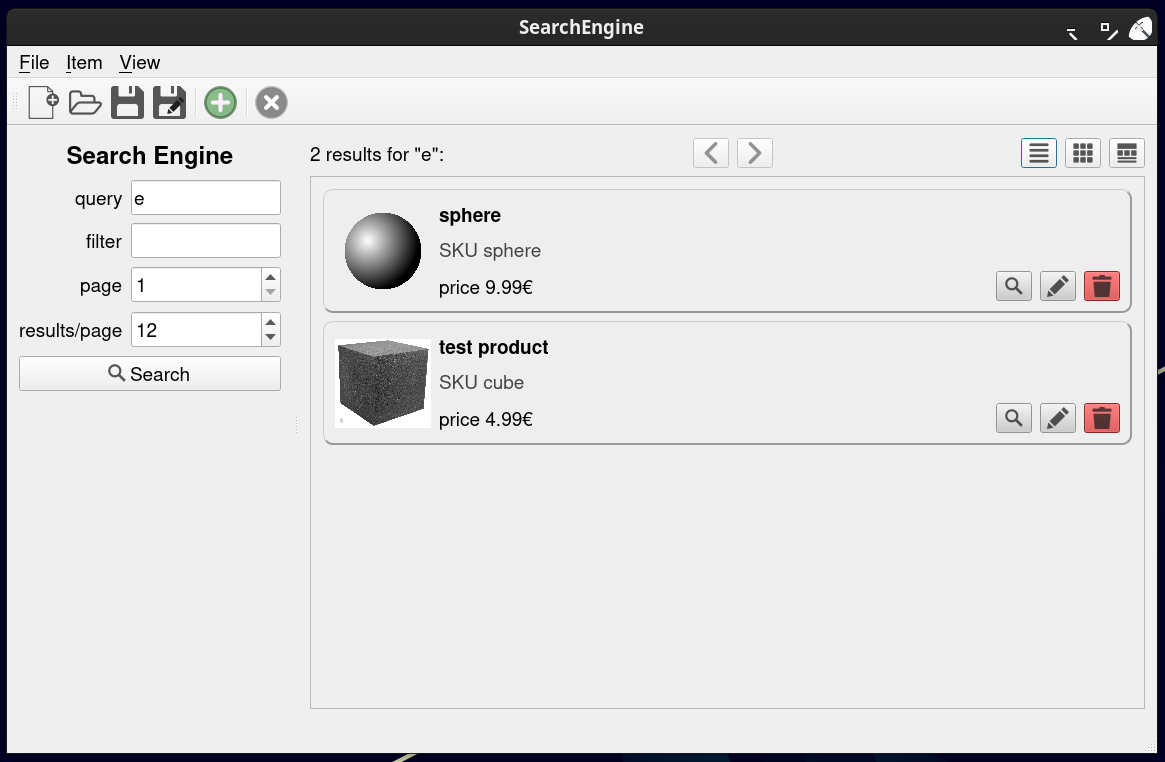
\includegraphics[height=0.55\textwidth]{assets/figure-search-engine-1}
 \end{center}
\end{frame}


\begin{frame}{Sketch}
 \begin{center}
  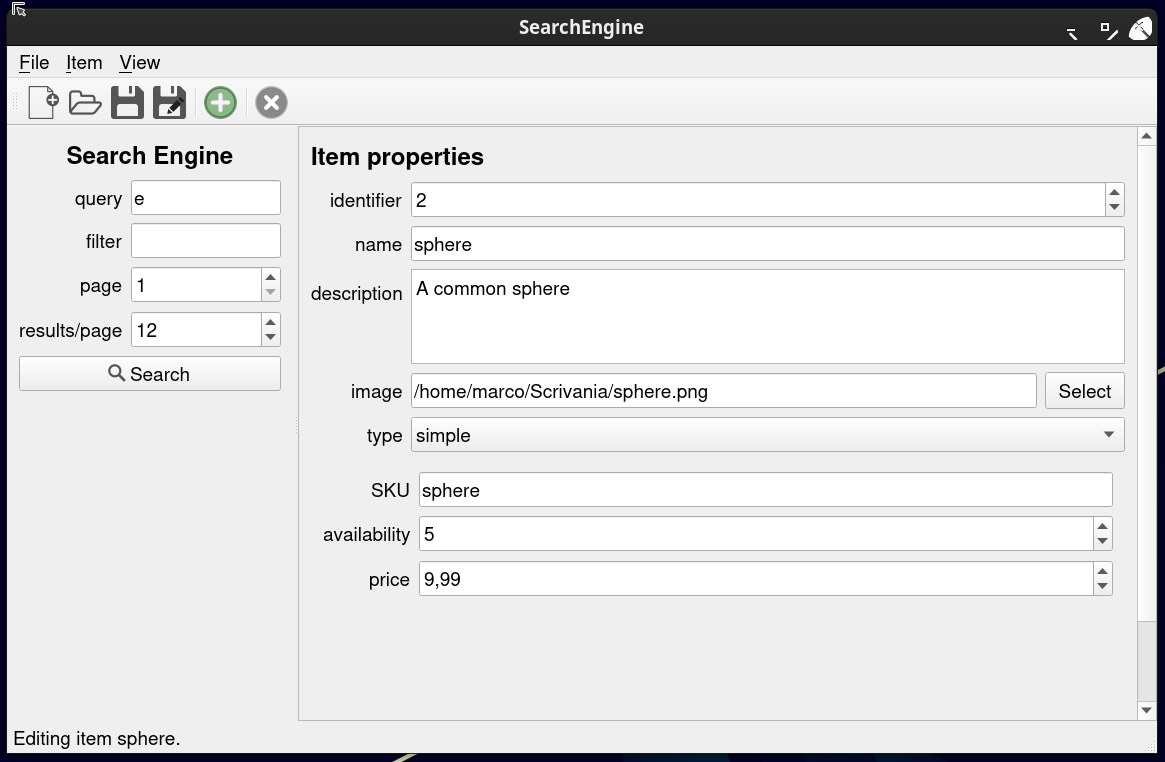
\includegraphics[height=0.55\textwidth]{assets/figure-search-engine-2}
 \end{center}
\end{frame}


%-----------------------------------------------------------------------
\section{Core Model Code}
\begin{frame}{Core Model Code}
 In this phase:
 
 \begin{itemize}
  \item plan \emph{classes}, attributes and functions (UML?)
  \item write \emph{code}
  \item run informal \emph{tests}
  \item repeat if necessary
 \end{itemize}
\end{frame}


\begin{frame}{Core Model Code / Classes}
 \begin{center}
  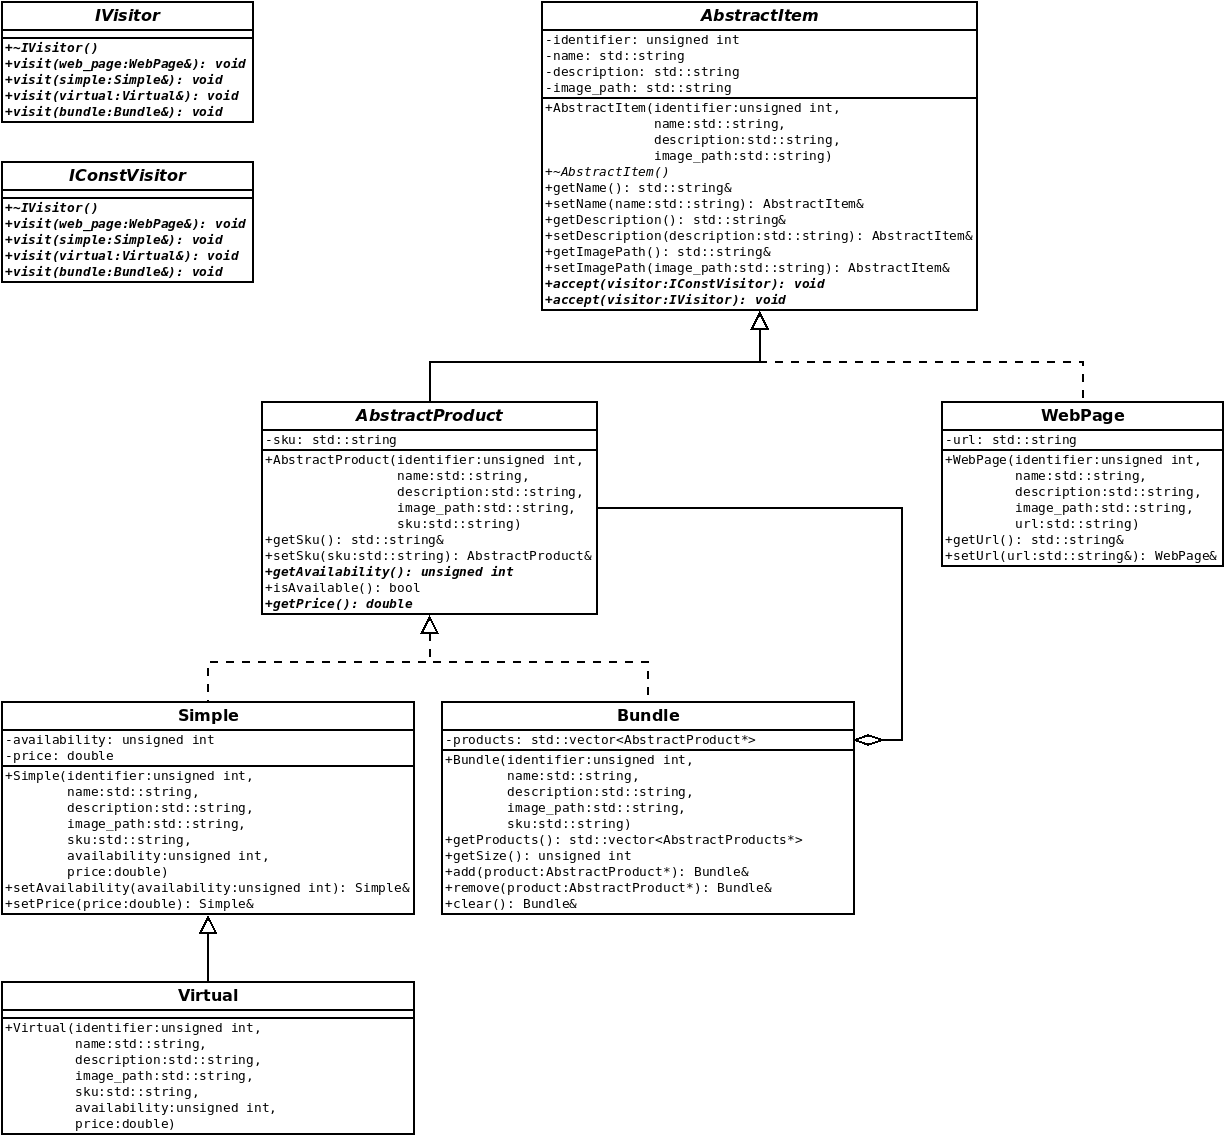
\includegraphics[height=0.61\textwidth]{assets/diagram-search-engine}
 \end{center}
\end{frame}


%-----------------------------------------------------------------------
\section{GUI Code}
\begin{frame}{GUI Code}
 In this phase:
 
 \begin{itemize}
  \item plan \emph{classes}, attributes and functions (UML?)
  \item write \emph{code}
  \item run informal \emph{tests}
  \item repeat if necessary
 \end{itemize}
 
 Same as the core model code.
\end{frame}


%-----------------------------------------------------------------------
\section{Refinement and Report}
\begin{frame}{Refinement and Report}
 In this phase:
 
 \begin{itemize}
  \item \emph{polish} the GUI
  \item draw final \emph{assets}
  \item prepare a \emph{meaningful dataset}
  \item write a convincing \emph{report}
 \end{itemize}
\end{frame}


\begin{frame}{Refinement and Report / Polish}
 Refinements to the GUI:
 
 \begin{itemize}
  \item tool-tips for buttons
  \item icons
  \item keyboard shortcuts
  \item colors and style
 \end{itemize}
\end{frame}


\begin{frame}{Refinement and Report / Assets}
 Final version of the assets:
 
 \begin{itemize}
  \item use adequate aspect ratio and resolution
  \item optimize weight (in KB)
  \item use colors which fit the GUI
  \item same for multimedia assets
 \end{itemize}
\end{frame}


\begin{frame}{Refinement and Report / Meaningful Dataset}
 A set of items which:
 
 \begin{itemize}
  \item is not too small
  \item is not too big
  \item allows to showcase features
  \item covers every functionality
 \end{itemize}
\end{frame}


\begin{frame}{Refinement and Report / Convincing Report}
 A good report should:
 
 \begin{itemize}
  \item let the reader quickly understand the subject
  \item keep personal and technical content separate
  \item use images when needed
  \item focus on the contribution
 \end{itemize}
\end{frame}


\begin{frame}{Source Code}
 \begin{columns}
  \begin{column}{0.15\textwidth}
   
\includegraphics[width=0.99\textwidth]{assets/logo-github}
  \end{column}
  \begin{column}{0.85\textwidth}
   Source code available at:
   \url{https://github.com/Unipd-Object-Oriented-Programming/search-engine}
  \end{column}
 \end{columns}
\end{frame}
\end{document}